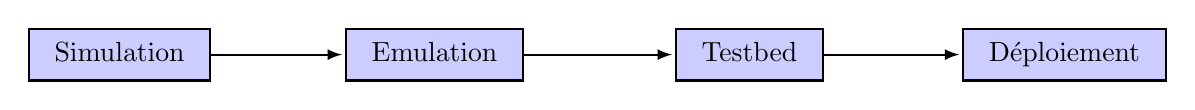
\begin{tikzpicture}[->,>=latex,shorten >=1pt,auto,node distance=3cm,
  thick,main node/.style={fill=blue!20,draw}]

  \node[main node] (sim) at (0,0) {\begin{tabular}{c}Simulation\end{tabular}};
  \node[main node] (emu) at (4,0) {\begin{tabular}{c}Emulation\end{tabular}};
  \node[main node] (iotlab) at (8,0) {\begin{tabular}{c}Testbed\end{tabular}};
  \node[main node] (final) at (12,0) {\begin{tabular}{c}Déploiement\end{tabular}};

  \path
    (sim) edge[] (emu)
    % (emu) edge [bend left=10] node[below] {Modèle} (sim)

    (emu) edge[] (iotlab)
    % (iotlab) edge [bend left=10] node[below] {Prototype} (emu)

    (iotlab) edge[] (final)
    % (final) edge [bend left=10] node[below] {Finalisation} (iotlab)

;
\end{tikzpicture}